% ==============================================================================
% CHƯƠNG 2: CƠ CHẾ BIỂU DIỄN TRI THỨC HÌNH HỌC VÀ ĐỒ THỊ TRI THỨC
% ==============================================================================

\chapter{CƠ CHẾ BIỂU DIỄN TRI THỨC HÌNH HỌC VÀ ĐỒ THỊ TRI THỨC}
\label{chap:representation}

\section{Ngôn ngữ Vị từ Hình học Phẳng (Geometric Predicate Language)}
Để máy tính có thể xử lý và suy diễn chính xác, toàn bộ các đối tượng và quan hệ hình học trong không gian Euclid hai chiều ($\mathbb{R}^2$) được hình thức hóa thành hệ thống vị từ bậc nhất (First-Order Predicates). 

\subsection{Phân loại Vị từ Cơ sở}
Hệ thống phân chia vị từ thành 4 nhóm chính:
\begin{enumerate}
    \item \textbf{Vị từ Đối tượng và Cấu hình Hình học}:
    \begin{itemize}
        \item $\text{Point}(A)$: Khai báo điểm $A$.
        \item $\text{Segment}(A, B)$: Khai báo đoạn thẳng nối $A$ và $B$ (có tính đối xứng $\text{Segment}(A, B) \equiv \text{Segment}(B, A)$).
        \item $\text{Triangle}(A, B, C)$: Tam giác tạo bởi 3 điểm không thẳng hàng $A, B, C$.
        \item $\text{RightTriangle}(A, B, C)$: Tam giác vuông tại $A$ ($\angle BAC = 90^\circ$).
        \item $\text{Quadrilateral}(A, B, C, D)$: Tứ giác lồi $ABCD$.
        \item $\text{Parallelogram}(A, B, C, D)$: Hình bình hành $ABCD$.
        \item $\text{Rhombus}(A, B, C, D)$: Hình thoi $ABCD$.
        \item $\text{Circle}(O)$: Đường tròn tâm $O$.
        \item $\text{CyclicQuadrilateral}(A, B, C, D, \text{Circle}(O))$: Tứ giác $ABCD$ nội tiếp đường tròn $(O)$.
    \end{itemize}
    
    \item \textbf{Vị từ Vị trí Tương đối và Cấu trúc Điểm}:
    \begin{itemize}
        \item $\text{Collinear}(A, B, C)$: Ba điểm $A, B, C$ thẳng hàng.
        \item $\text{Midpoint}(M, AB)$: Điểm $M$ là trung điểm của đoạn thẳng $AB$.
        \item $\text{IntersectionPoint}(P, AB, CD)$: Điểm $P$ là giao điểm của hai đoạn thẳng $AB$ và $CD$.
        \item $\text{PointOnCircle}(P, \text{Circle}(O))$: Điểm $P$ nằm trên đường tròn $(O)$ ($OP = R$).
        \item $\text{PointOutsideCircle}(M, \text{Circle}(O))$: Điểm $M$ nằm ngoài đường tròn $(O)$ ($OM > R$).
        \item $\text{TangentSegment}(M, A, \text{Circle}(O))$: Đoạn thẳng $MA$ là tiếp tuyến với đường tròn $(O)$ tại tiếp điểm $A$ ($OA \perp MA$).
        \item $\text{SecantSegment}(M, C, D, \text{Circle}(O))$: Đường thẳng $MCD$ là cát tuyến cắt $(O)$ tại hai điểm $C$ và $D$.
        \item $\text{Foot}(H, A, BC)$: Điểm $H$ là hình chiếu vuông góc của $A$ lên đường thẳng $BC$ ($AH \perp BC$ và $H \in BC$).
    \end{itemize}

    \item \textbf{Vị từ Quan hệ Hình học Nhị phân}:
    \begin{itemize}
        \item $\text{Parallel}(AB, CD)$: Đoạn thẳng $AB$ song song với $CD$.
        \item $\text{Perpendicular}(AB, CD)$: Đoạn thẳng $AB$ vuông góc với $CD$.
        \item $\text{Congruent}(AB, CD)$: Đoạn thẳng $AB$ bằng đoạn thẳng $CD$ ($|AB| = |CD|$).
        \item $\text{CongruentTriangles}(ABC, DEF)$: Hai tam giác bằng nhau ($\triangle ABC \cong \triangle DEF$).
        \item $\text{SimilarTriangles}(ABC, DEF)$: Hai tam giác đồng dạng ($\triangle ABC \sim \triangle DEF$).
        \item $\text{Concurrent}(d_1, d_2, d_3)$: Ba đường thẳng $d_1, d_2, d_3$ đồng quy tại một điểm.
    \end{itemize}

    \item \textbf{Vị từ Đại số và Đo lường}:
    \begin{itemize}
        \item $\text{Equal}(\text{Angle}(ABC), 60)$: Góc $\angle ABC$ có số đo bằng $60^\circ$.
        \item $\text{Equal}(\text{Length}(AB), 5)$: Đoạn thẳng $AB$ có độ dài bằng 5.
        \item $\text{Equal}(\text{Pow}(\text{Length}(MA), 2), \text{Mul}(\text{Length}(MC), \text{Length}(MD)))$: Hệ thức đại số $MA^2 = MC \cdot MD$.
    \end{itemize}
\end{enumerate}

\section{Mô hình Đồ thị Tri thức Hình học trên Neo4j (Knowledge Graph)}
Toàn bộ tri thức hình học phẳng, từ các khái niệm cơ sở (Ontology Classes) đến hệ thống định lý và tiên đề, được tổ chức dưới dạng một Đồ thị Thuộc tính Lớn (Property Graph) lưu trữ trên cơ sở dữ liệu đồ thị bản địa \textbf{Neo4j}.

\subsection{Cấu trúc Lược đồ Đồ thị (Schema Design)}
\begin{itemize}
    \item \textbf{Nút (Nodes)}:
    \begin{itemize}
        \item \texttt{Rule}: Biểu diễn một quy tắc suy diễn hoặc định lý toán học (thuộc tính: \texttt{id}, \texttt{name}, \texttt{domain}, \texttt{description}, \texttt{formula}).
        \item \texttt{Fact}: Biểu diễn một tiên đề vị từ hoặc sự kiện mẫu (thuộc tính: \texttt{id}, \texttt{value}, \texttt{label}).
        \item \texttt{OntologyClass}: Biểu diễn phân cấp khái niệm (ví dụ: \texttt{Polygon}, \texttt{Triangle}, \texttt{RightTriangle}, \texttt{Circle}).
        \item \texttt{FormalGeo}: Định danh các định lý kế thừa từ thư viện FormalGeo.
    \end{itemize}
    \item \textbf{Quan hệ (Edges / Relationships)}:
    \begin{itemize}
        \item \texttt{HAS\_INPUT}: Nối từ nút \texttt{Rule} tới các nút \texttt{Fact} điều kiện tiền đề.
        \item \texttt{HAS\_OUTPUT}: Nối từ nút \texttt{Rule} tới các nút \texttt{Fact} kết luận suy ra.
        \item \texttt{IS\_A}: Phân cấp kế thừa giữa các lớp đối tượng (ví dụ: \texttt{RightTriangle} $\xrightarrow{\text{IS\_A}}$ \texttt{Triangle} $\xrightarrow{\text{IS\_A}}$ \texttt{Polygon}).
        \item \texttt{INSTANCE\_OF}: Nối một thực thể hình học cụ thể với lớp khái niệm của nó.
    \end{itemize}
\end{itemize}

\begin{figure}[h!]
\centering
\begin{subfigure}[b]{0.48\textwidth}
    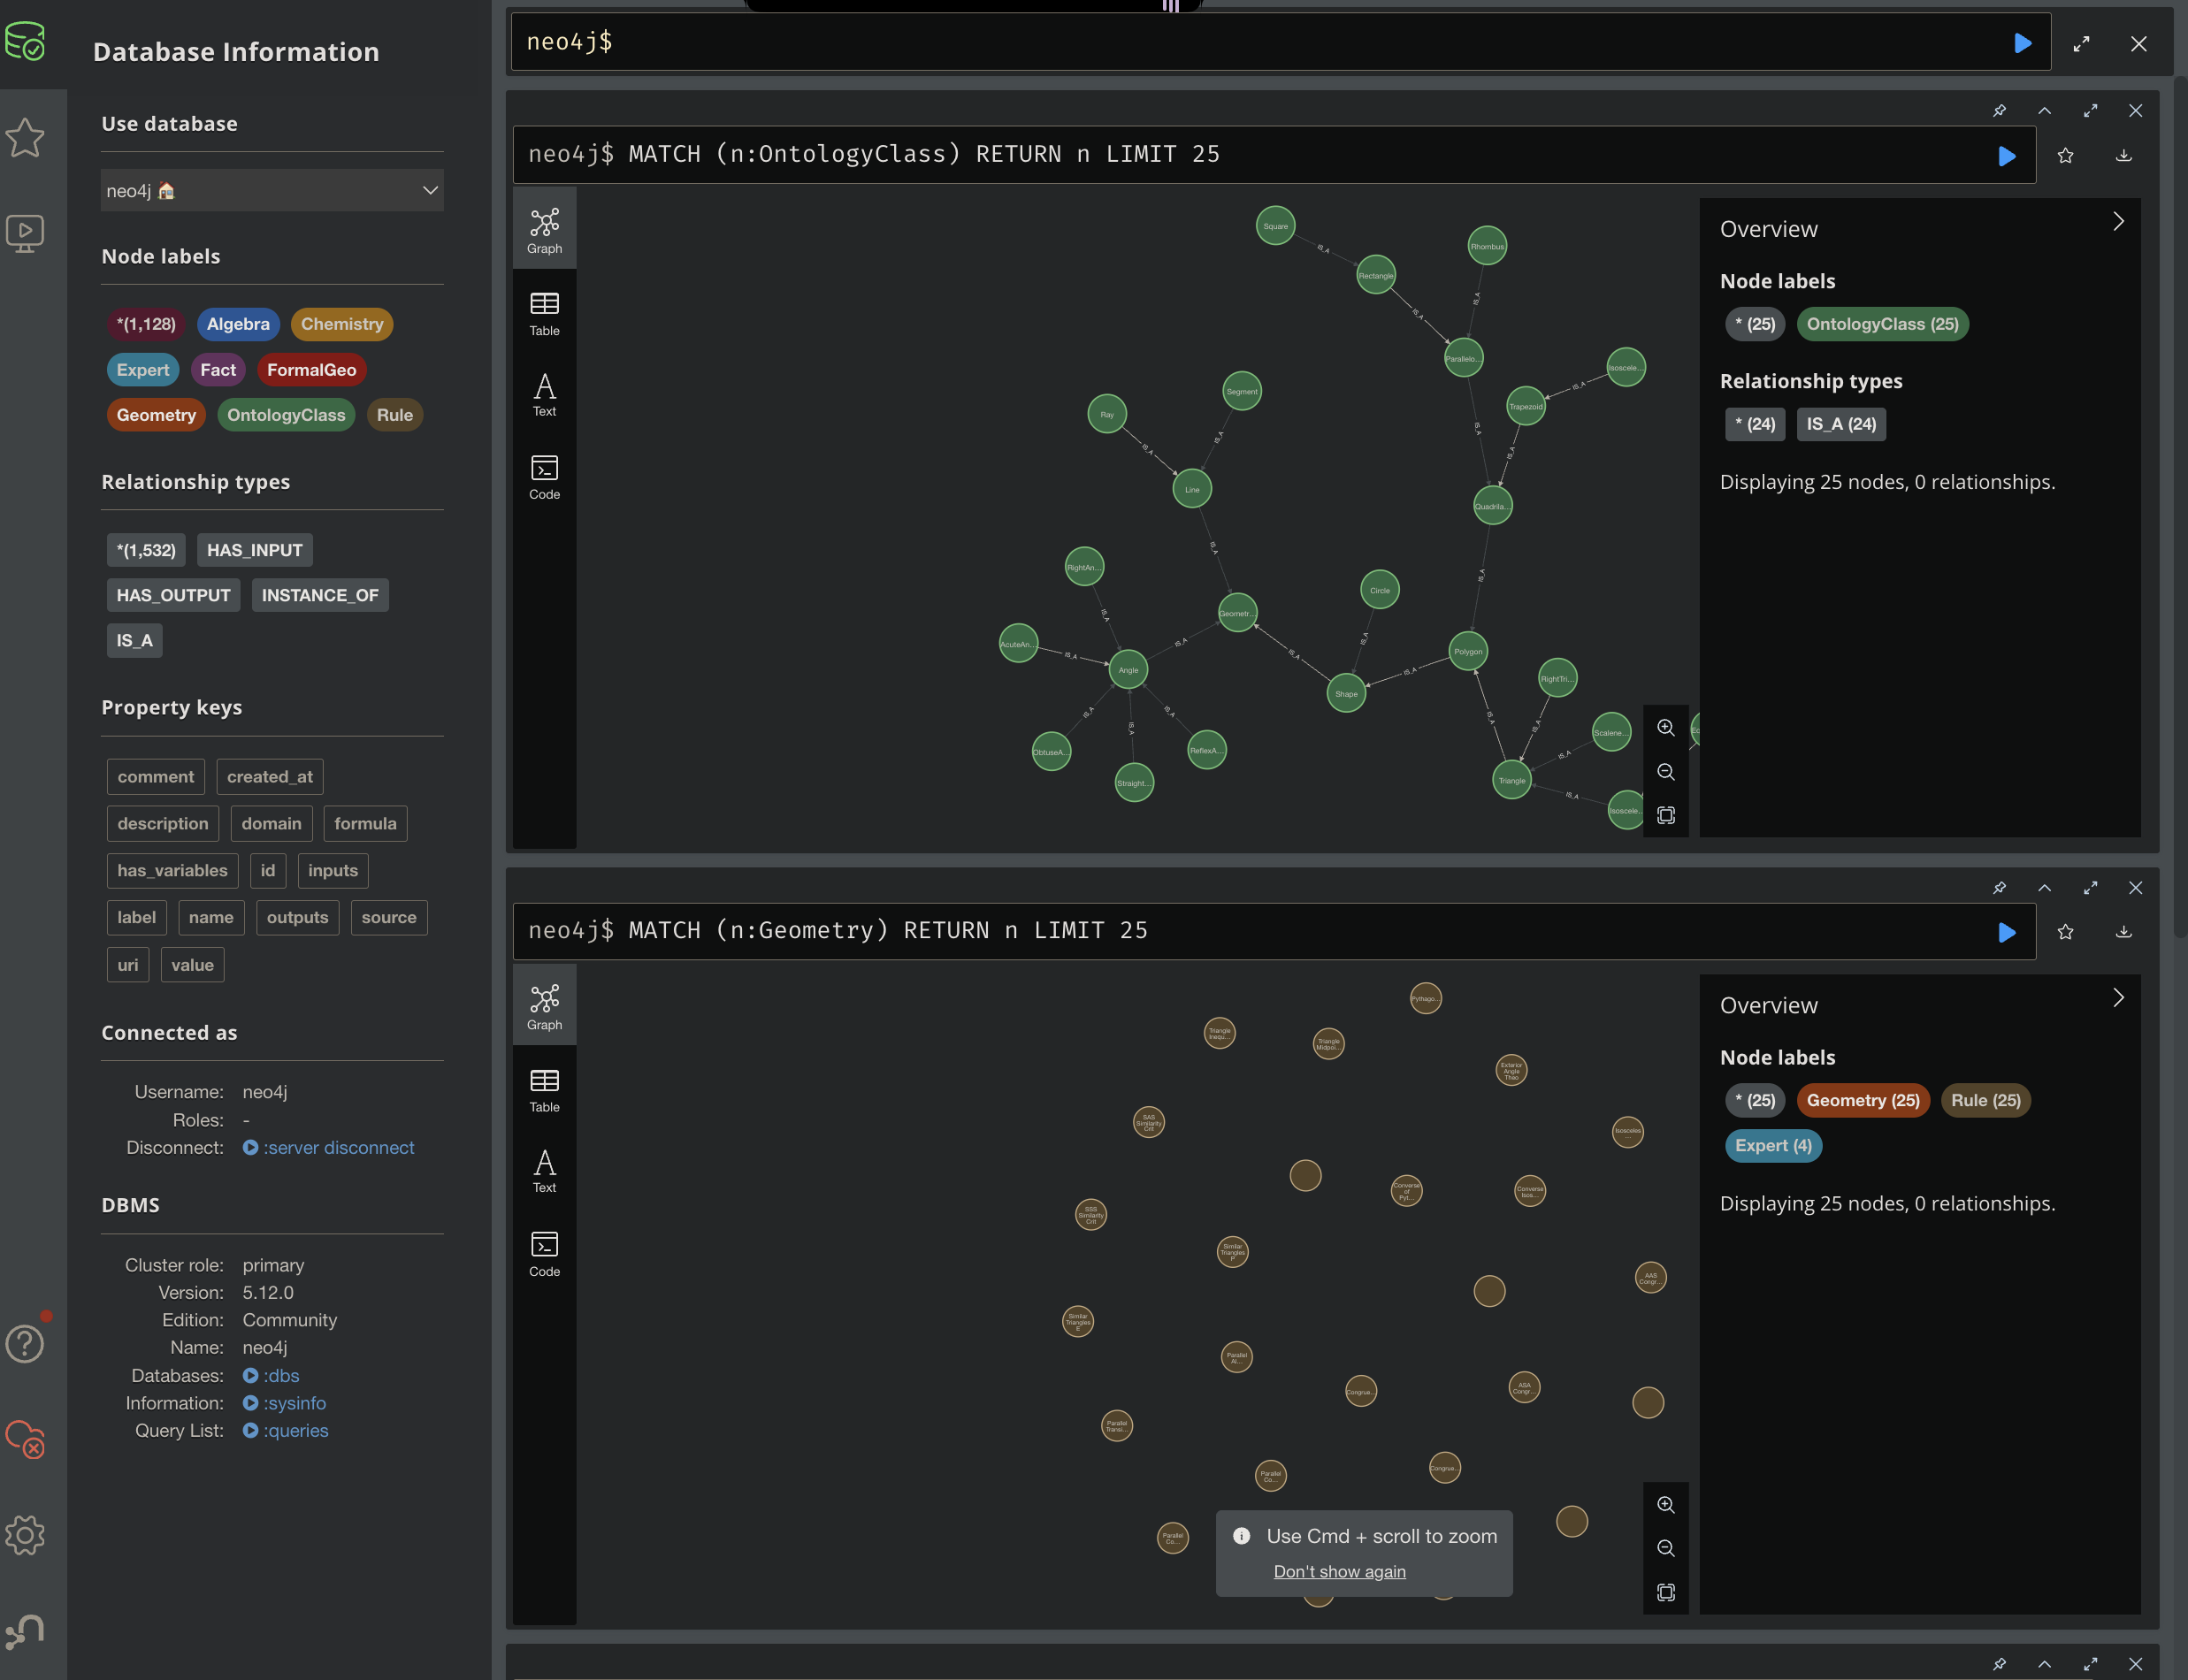
\includegraphics[width=\textwidth]{../assets/neo4j_full_ontology_1128_nodes.png}
    \caption{Thống kê toàn bộ Ontology trên Neo4j (1.128 nút, 1.532 quan hệ).}
    \label{fig:neo4j_ontology_stats}
\end{subfigure}
\hfill
\begin{subfigure}[b]{0.48\textwidth}
    \includegraphics[width=\textwidth]{../assets/neo4j_knowledge_base.png}
    \caption{Trực quan hóa mạng lưới kết nối giữa các định lý và tiên đề.}
    \label{fig:neo4j_graph_view}
\end{subfigure}
\caption{Cơ sở Tri thức Đồ thị Hình học Phẳng được xây dựng và truy vấn trên Neo4j.}
\label{fig:neo4j_full_kb}
\end{figure}

Như thể hiện trong Hình~\ref{fig:neo4j_ontology_stats}, cơ sở tri thức đã được nạp đầy đủ \textbf{1.128 nút} và \textbf{1.532 quan hệ}, bao quát toàn diện các nhánh tri thức:
\begin{itemize}
    \item \textbf{Nhóm Tiên đề Euclid Cơ bản}: Quan hệ cộng góc, cộng đoạn thẳng, góc đối đỉnh, góc so le trong, góc đồng vị, các trường hợp bằng nhau của tam giác ($c-c-c, c-g-c, g-c-g$).
    \item \textbf{Nhóm Định lý Tam giác \& Tứ giác}: Định lý Pythagore, Định lý Thales, đường trung bình, tính chất trọng tâm, trực tâm, tâm đường tròn nội/ngoại tiếp, tính chất hình thoi, hình bình hành, tứ giác nội tiếp.
    \item \textbf{Nhóm Định lý Đường tròn Nâng cao}: Góc nội tiếp, góc tạo bởi tiếp tuyến và dây cung, phương tích của một điểm đối với đường tròn (Định lý cát tuyến - tiếp tuyến $PT^2 = PA \cdot PB$, Định lý hai dây cung cắt nhau $PA \cdot PB = PC \cdot PD$).
    \item \textbf{Nhóm Định lý Olympic (IMO)}: Định lý Ptolemy cho tứ giác nội tiếp, Định lý Ceva, Định lý Menelaus, Định lý đường thẳng Simson, Định lý Varignon cho trung điểm tứ giác, Bổ đề điểm Nagel.
\end{itemize}

\section{Cơ sở Dữ liệu Vector Qdrant và Cơ chế GraphRAG}
Để giải quyết bài toán tìm kiếm định lý phù hợp từ ngôn ngữ tự nhiên hoặc từ tập sự kiện phức tạp mà không phụ thuộc vào chuỗi ký tự cứng nhắc (Exact Keyword Matching), hệ thống sử dụng \textbf{Qdrant Cloud Vector Database} làm động cơ tìm kiếm tương đồng ngữ nghĩa (Dense Semantic Search).

\begin{figure}[h!]
\centering
\begin{subfigure}[b]{0.48\textwidth}
    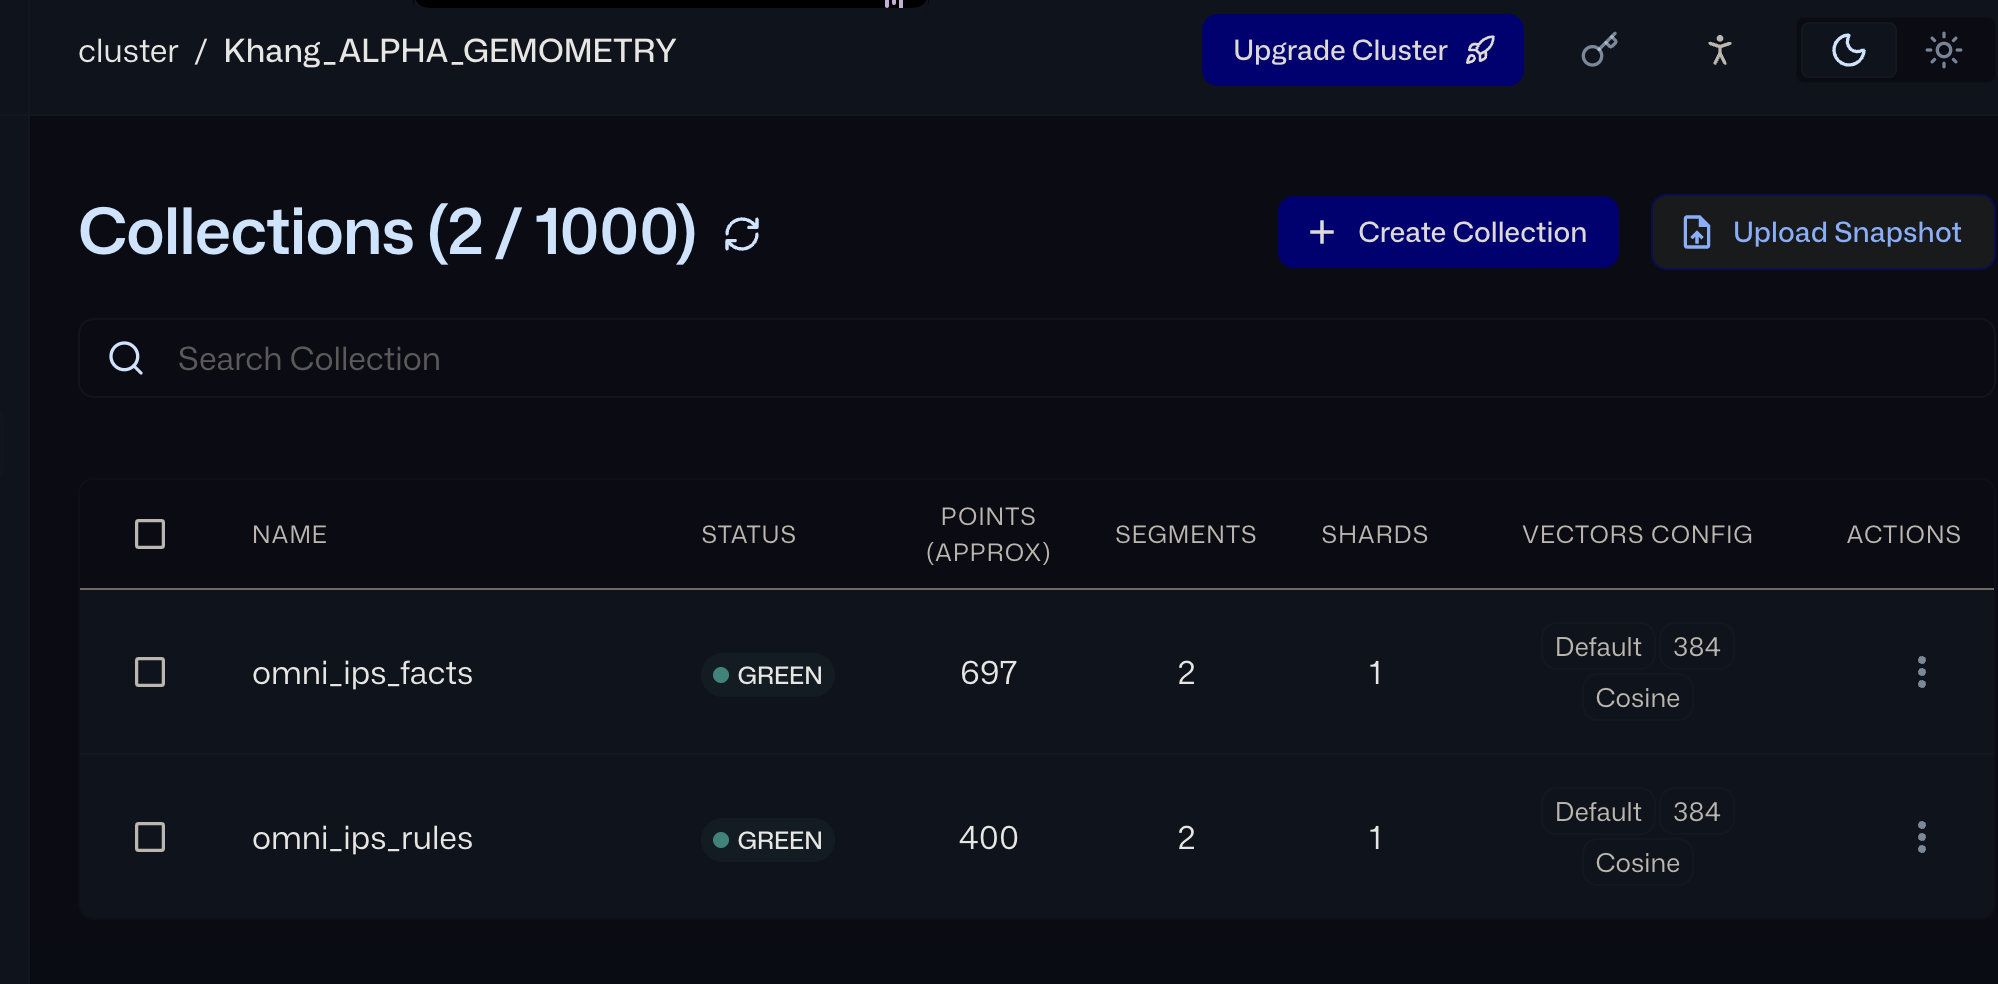
\includegraphics[width=\textwidth]{../assets/qdrant_collections_overview.png}
    \caption{Tổng quan các Collections được lập chỉ mục vector trên Qdrant.}
    \label{fig:qdrant_collections}
\end{subfigure}
\hfill
\begin{subfigure}[b]{0.48\textwidth}
    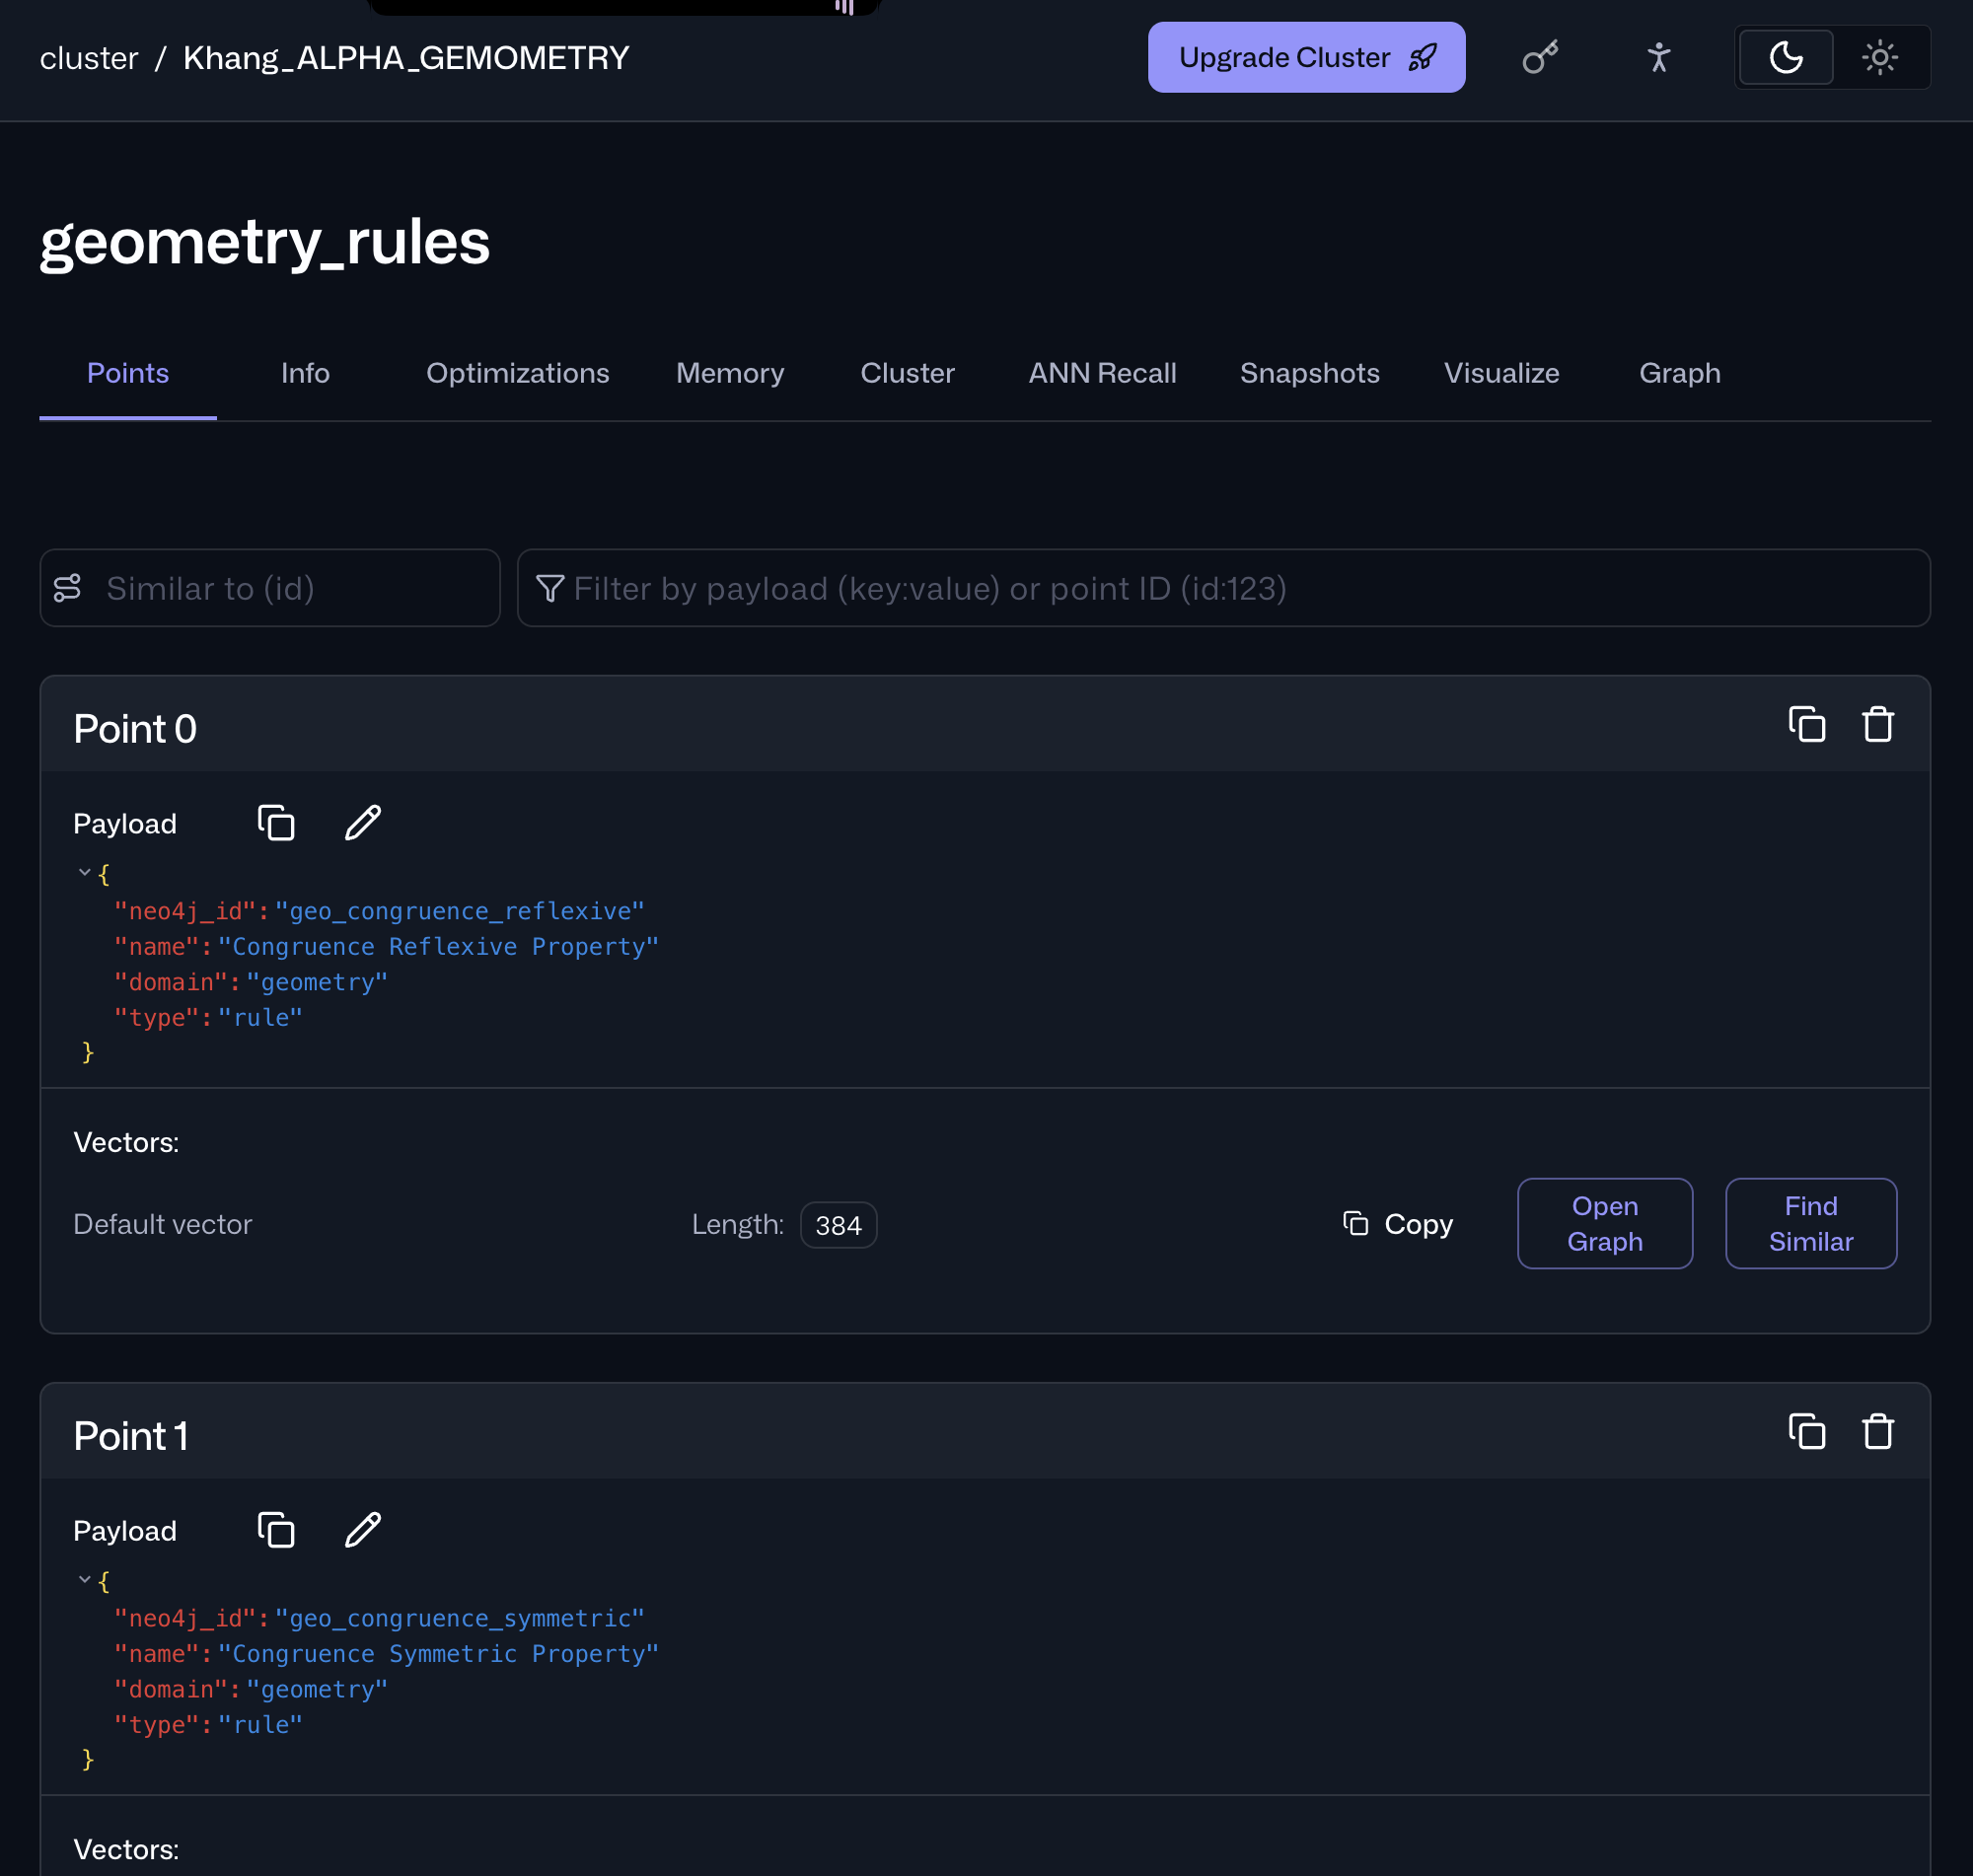
\includegraphics[width=\textwidth]{../assets/qdrant_rules_payload_detail.png}
    \caption{Cấu trúc Payload chi tiết của một định lý hình học trong Qdrant.}
    \label{fig:qdrant_rules_payload}
\end{subfigure}
\caption{Quản lý và lập chỉ mục không gian vector tri thức hình học trên Qdrant Cloud.}
\label{fig:qdrant_management}
\end{figure}

\subsection{Cấu trúc Chỉ mục Vector trong Qdrant}
Như minh họa trong Hình~\ref{fig:qdrant_collections}, hệ thống duy trì hai collection vector chính:
\begin{enumerate}
    \item \texttt{omni\_ips\_rules} (hoặc \texttt{geometry\_rules}): Lưu trữ các định lý và quy tắc suy diễn hình học. Mỗi vector đại diện cho mô tả ngữ nghĩa, công thức toán học và tiền đề của một luật. Payload chứa định danh Neo4j (\texttt{neo4j\_id}), mô tả và mã luật tương ứng (Hình~\ref{fig:qdrant_rules_payload}).
    \item \texttt{omni\_ips\_facts} (hoặc \texttt{geometry\_facts}): Lưu trữ các dạng biểu diễn vị từ thực tế của các sự kiện hình học, hỗ trợ ánh xạ nhanh các câu khẳng định tự nhiên sang vị từ chuẩn (Hình~\ref{fig:qdrant_facts_payload}).
\end{enumerate}

\begin{figure}[h!]
\centering
\begin{subfigure}[b]{0.48\textwidth}
    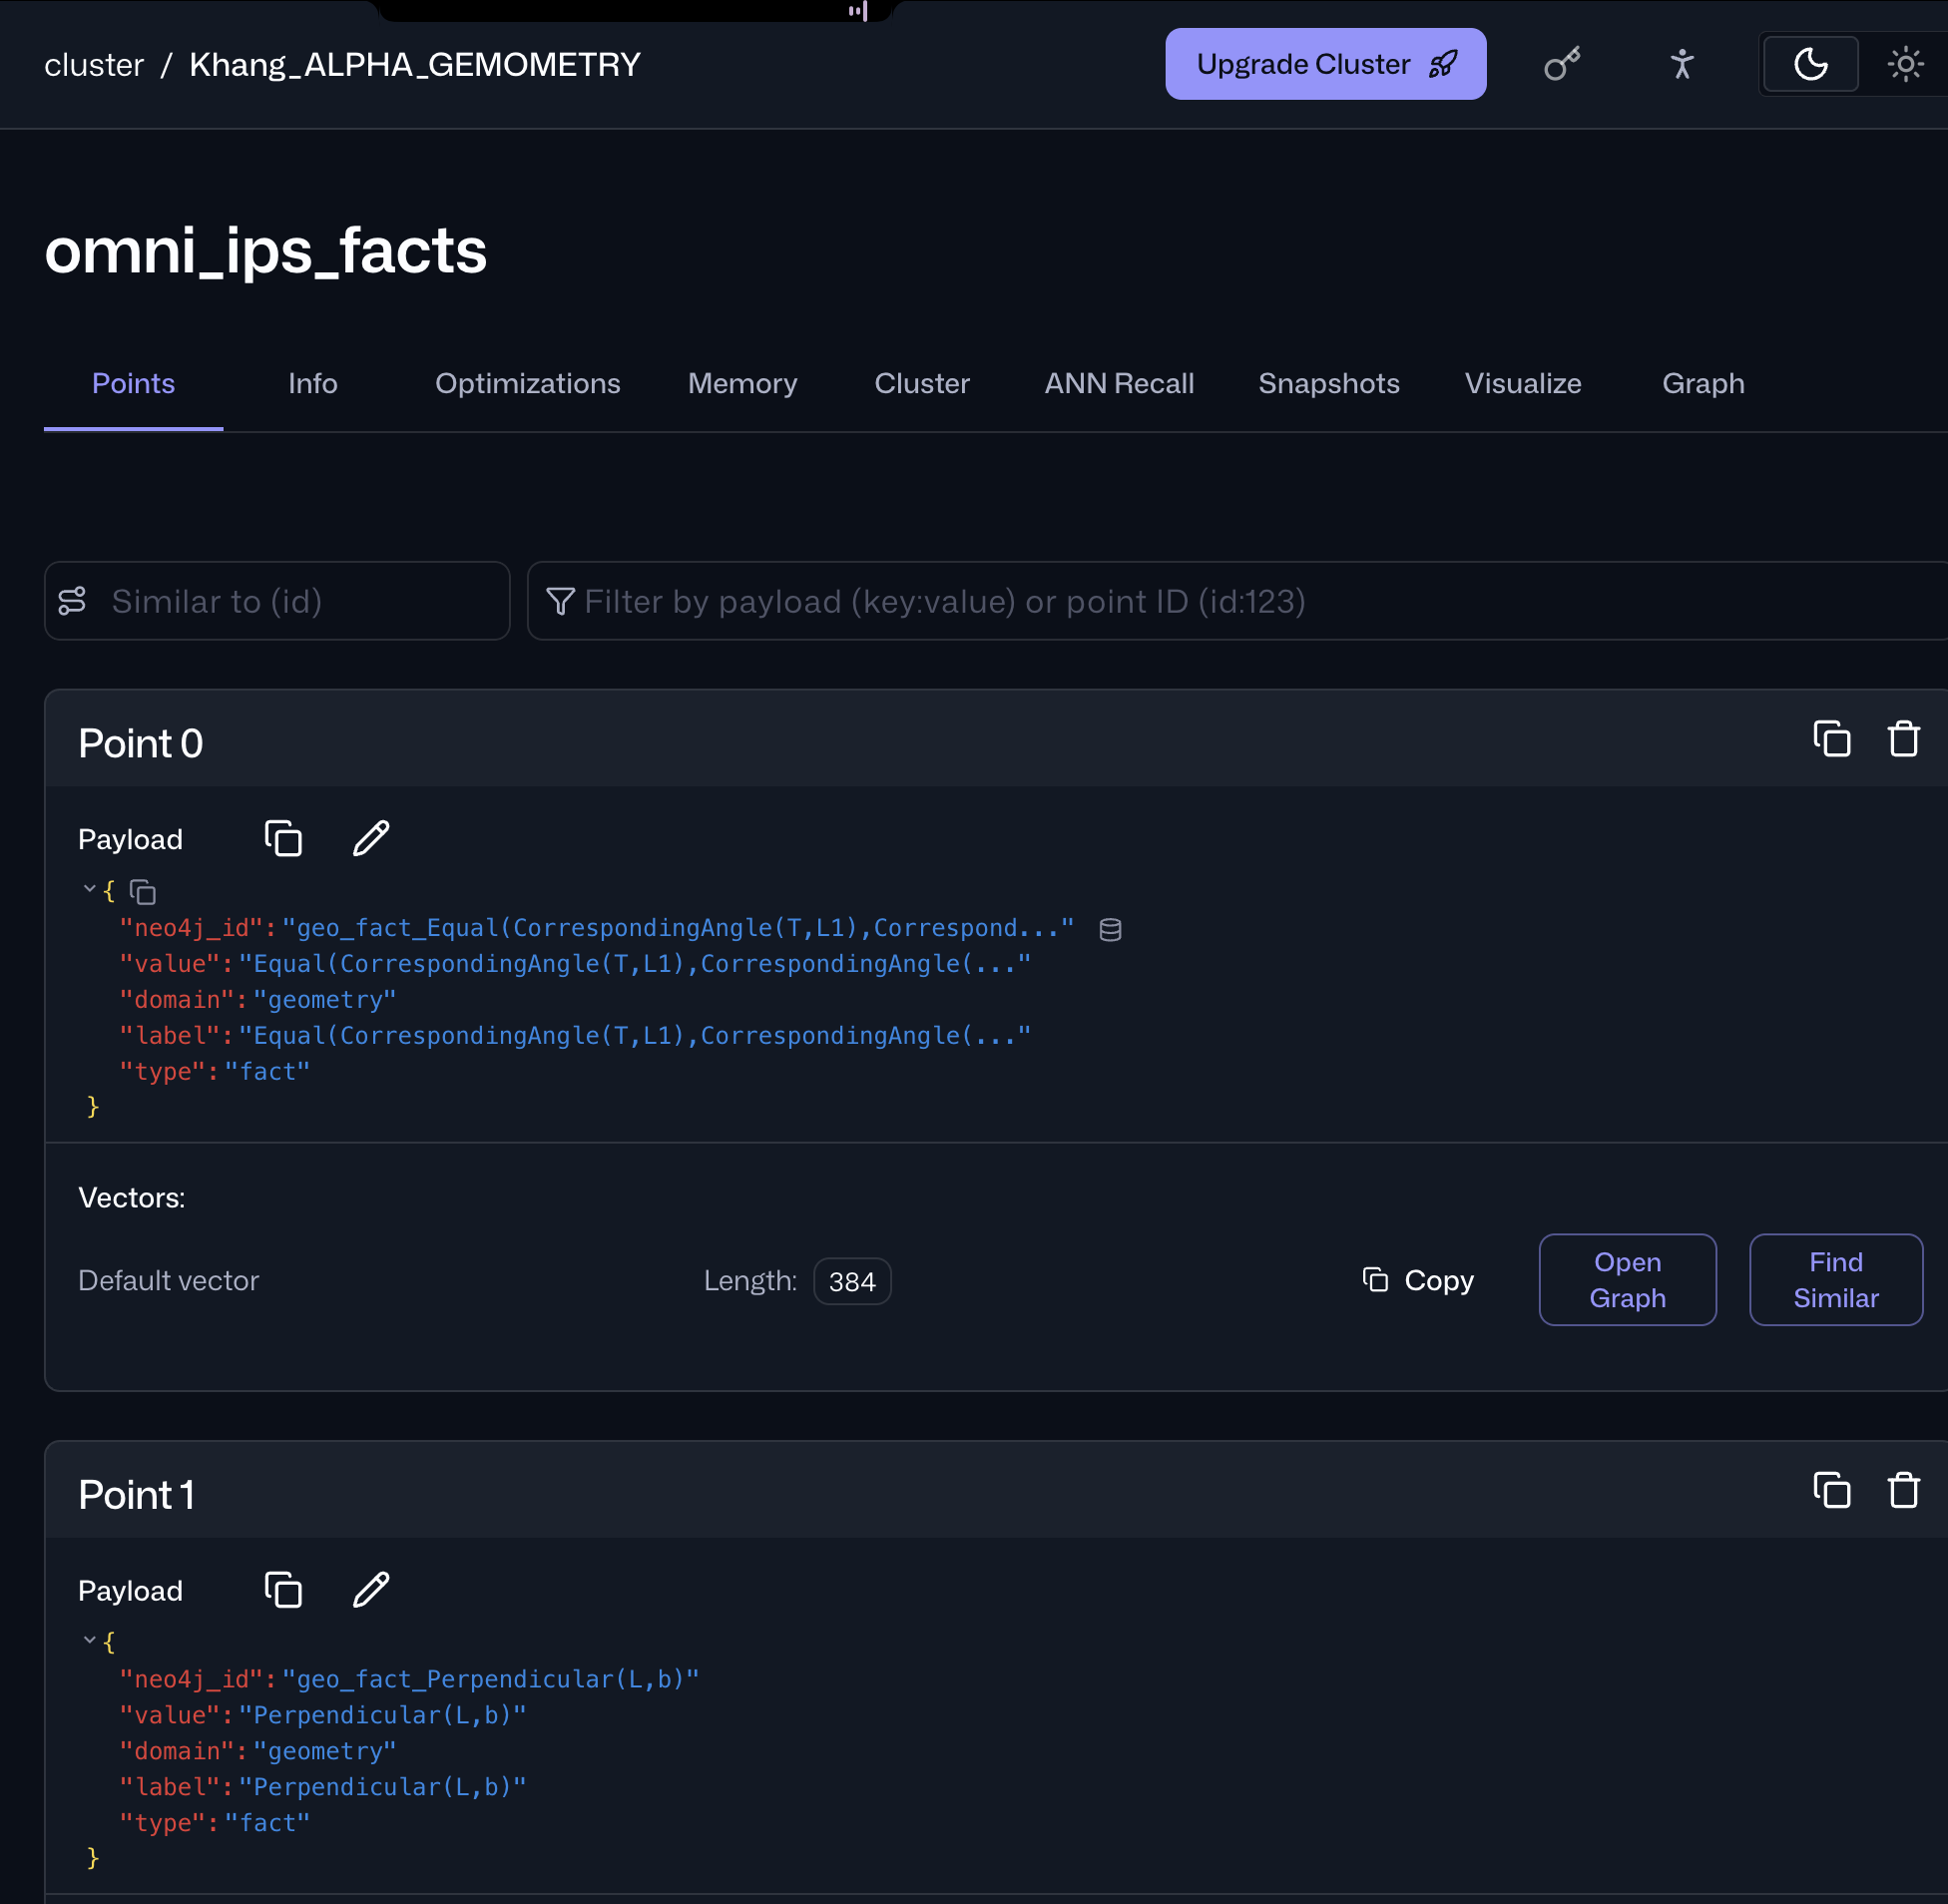
\includegraphics[width=\textwidth]{../assets/qdrant_facts_payload_detail.png}
    \caption{Payload vị từ sự kiện hình học trong \texttt{omni\_ips\_facts}.}
    \label{fig:qdrant_facts_payload}
\end{subfigure}
\hfill
\begin{subfigure}[b]{0.48\textwidth}
    \includegraphics[width=\textwidth]{../assets/qdrant_vector_db.png}
    \caption{Truy vấn tương đồng vector điểm sự kiện \texttt{Midpoint(N,AC)}.}
    \label{fig:qdrant_vector_search}
\end{subfigure}
\caption{Chi tiết lưu trữ sự kiện và không gian vector trên Qdrant.}
\label{fig:qdrant_details}
\end{figure}

\section{Bộ Định tuyến Neuro-Symbolic và Trích xuất Vị từ từ Đề bài}
Một mắt xích tối quan trọng trong hệ thống là quá trình chuyển đổi (Parsing) đề bài bài toán từ ngôn ngữ tự nhiên tiếng Việt (kèm theo mã công thức LaTeX) sang tập hợp các vị từ ban đầu (Initial Facts) và mục tiêu cần chứng minh (Goal).

\subsection{Quy trình Xử lý Vị từ Đa tầng (Multi-Stage Parsing Pipeline)}
\begin{enumerate}
    \item \textbf{Tầng 1: Bộ Tiền Xử lý và Làm sạch Toán học (\texttt{clean\_geometry\_query})}:
    Tự động chuẩn hóa các ký tự LaTeX dính liền hoặc biểu thức OCR lỗi từ việc copy-paste đề bài:
    $$\text{((O))} \longrightarrow \text{O}, \quad \text{\textbackslash cdot} \longrightarrow *, \quad \text{\textbackslash perp} \longrightarrow \text{vuông góc}, \quad \text{đoạn thẳng (MA, MB)} \longrightarrow \text{MA, MB}$$
    
    \item \textbf{Tầng 2: Direct JSON Schema Prompting qua LLM}:
    Thay vì sử dụng Function Calling (vốn dễ gây ra lỗi $400\ \text{tool\_use\_failed}$ trên các endpoint suy luận), hệ thống truyền trực tiếp lược đồ JSON nghiêm ngặt vào \texttt{SystemMessage} của mô hình ngôn ngữ lớn (Llama-3.3-70B / DeepSeek / GPT-OSS-120B). Đầu ra được trích xuất bằng regex JSON block an toàn với thời gian phản hồi cực nhanh ($< 1.8\text{s}$).

    \item \textbf{Tầng 3: Bộ Phân tích Dự phòng Offline (Regex Fallback Parser)}:
    Trong trường hợp mất kết nối mạng hoặc LLM quá tải, bộ phân tích Regex cục bộ sẽ tự động quét các từ khóa hình học đặc thù để trích xuất đầy đủ các vị từ: tam giác vuông, tiếp tuyến, cát tuyến, trung điểm, đường cao và tứ giác nội tiếp.
\end{enumerate}
